\documentclass[journal,10pt,twoside, a4paper]{IEEEtran}
\usepackage{cite,graphicx,array,color,amssymb,balance}
\usepackage[cmex10]{amsmath}


\title{Machine learning aided DSP in optical coherent receivers}

\author{
    \IEEEauthorblockN{L.H.P. Driessen\\}
    \IEEEauthorblockA{l.h.p.driessen@student.tue.nl, ID 0962549}
    \thanks{
        Supervisors: Patty Stabile, Chigo Okonkwo
    }
}
\begin{document}
\maketitle

\begin{abstract}
    A recurrent neural network has been used as a substitution to (parts of) the DSP chain in optical coherent receivers. Results with simulated data show that this technique not yet comparable to conventional filtering techniques. An accuracy of 98.5952\% (BER of $\mathbf{1.408\cdot 10^{-2}}$) has been achieved in simulated QPSK data with an SNR of 15 and a transmission differential group delay of 40ps. In real, frequency-offset compensated, 8-QAM data, an accuracy of 83.2145\% (BER of $\mathbf{1,67855\cdot 10^{-1}}$) has been achieved.
\end{abstract}

\section{Introduction}
\IEEEPARstart{F}{iber-optic} communication has replaced lots of the electrical communication in the last decades due to its lower interference and higher bandwidth. Conventionally, direct-detection with on-off keying was used in optical communication. In this scheme, the transmitting laser turns on or off depending on the information to be sent. This technique is easy to realize due to its simplistic nature. However, it is possible to achieve a greater bandwidth by using a coherent communication system\cite{coherent_detection,DSP_beyond}. Latest developments in coherent optical transmission have shown data communication rates in the Tb/s range\cite{coherent_detection, DSP_beyond, dsp+ml}.

Coherent optical fiber communication has been studied in the 1980s. The main advantage was to extend the communication length compared to conventional direct-detection communication\cite{coherent_detection}. In the 1990s and the beginning of the 2000s, research on coherent detection decreased to the advent of wavelength division multiplexing (WDM). Research on coherent systems continued in 2005, which showed promising results\cite{continue}. The main advantage of coherent systems is that it benefits not only from light intensity, but also utilizes information such as light polarization and phase. This makes it suitable to deploy higher order modulations like QPSK and QAM, which results in higher data transmission rates. Using this information comes at the cost of higher complexity. It requires extra hardware to convert the signal to the electrical domain, as detection of polarization and phase of light is not feasible to do in the optical domain\cite{coherent_detection}. Digital signal processing (DSP) is used to recover the polarization, intensity and phase of the signal. Also, signal impairments due to channel imperfections can be compensated by DSP\cite{coherent_detection, DSP_2, DSP_beyond}. Some of these impairments, like polarization mode dispersion (PMD), are stochastic\cite{nonlinear} and have so far been compensated by linear filters. However, different approaches might be able to show other results.

A different approach to recover received optical signals might be to aid the DSP with machine learning methods. This is because machine learning techniques have proven to be useful in solving complex statistical problems. Different parts in the receiver sequence could be substituted by these techniques to enhance the receiver DSP performance. In this paper, the proof of concept of machine learning aided DSP in optical coherent receivers is provided and its feasibility is analyzed.

The structure of this document is as follows: in the next chapter, optical coherent communication is explained. Relevant machine learning techniques are explained in chapter 3. In chapter 4, it is discussed how different parts of the communication system can be replaced by machine learning. The simulated results are shown in chapter 5 and discussed in chapter 6. Finally, a conclusion is given in chapter 7.

\section{Fiber-optic coherent communication}
The overall system structure in optical coherent communication is depicted schematically in Fig.~\ref{fig:coherent_detection}. The transmitter subsystem is colored blue and the receiver part red. A optical fiber is placed in between the two subsystems. The use of multiple wavelengths (WDM) is omitted as this does not affect the general structure of both transmitter and receiver. The transmitter, medium and receiver are discussed next. After that, the DSP part of the receiver is addressed separately.
\begin{figure}
    \centering
    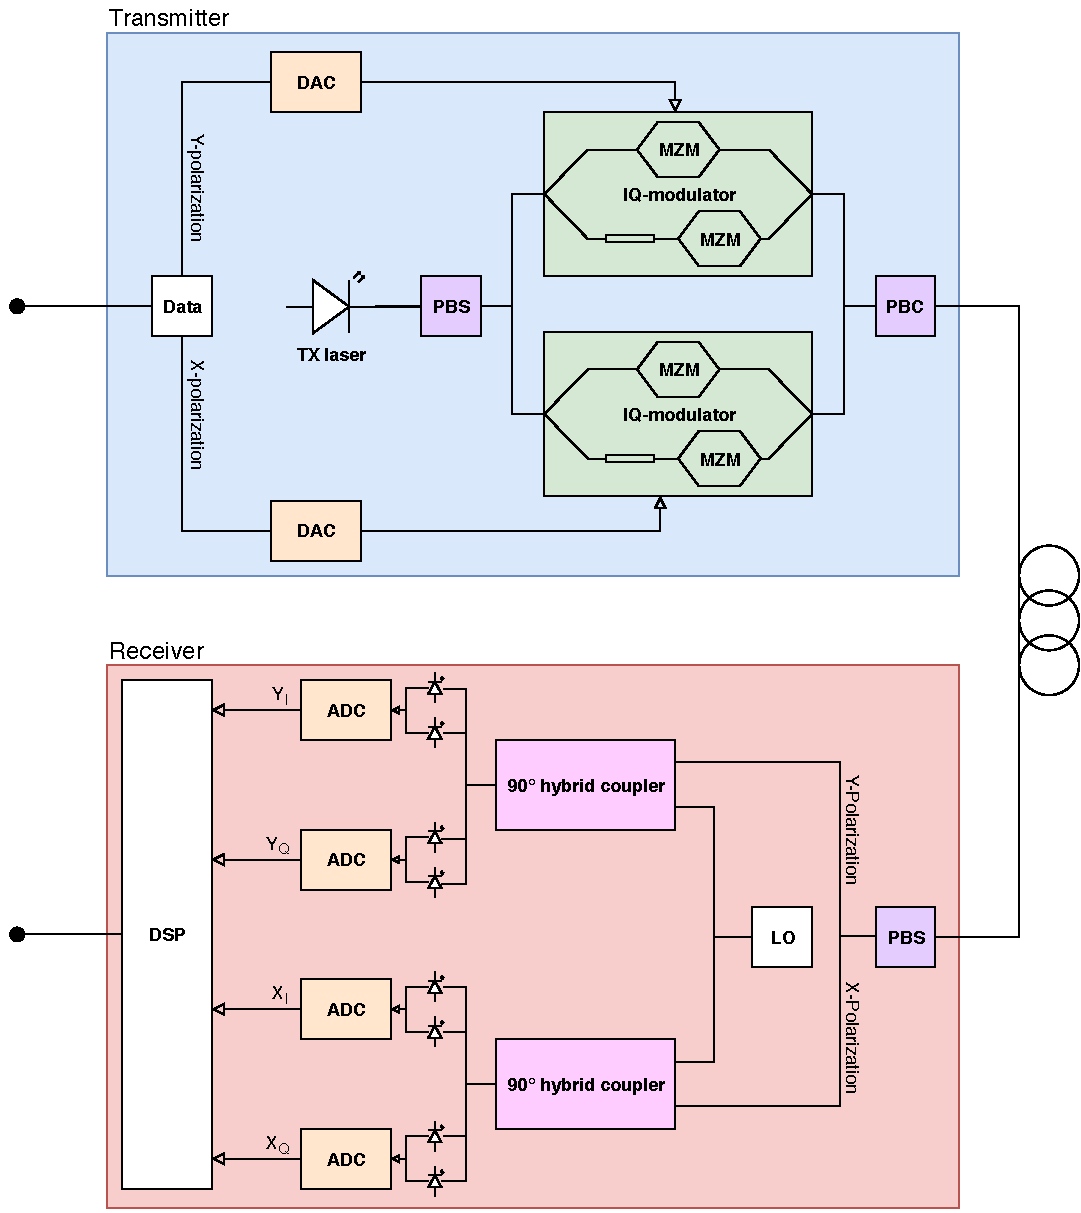
\includegraphics[width=\linewidth]{images/coherent_detection}
    \caption{Schematic representation of an optical coherent detection system}
    \label{fig:coherent_detection}
\end{figure}
\subsection{Transmitter}
The transmitter in an optical coherent system consists of a continuous wave (CW) laser with a small linewidth. This laser is sent through a polarizing beam splitter (PBS), which splits the incoming light into two orthogonal linear polarized beams. 

The two beams are fed into in-phase and quadrature (IQ) modulators, which main function is to encode data onto the linear polarized beam. This data comes first goes through a digital to analog converter (DAC) and is sent into the IQ modulators. These IQ modulator are realized by substrates of $LiNbO_3$ or $InP$, which change their refractive indices linearly depending on the applied voltage. This effect is called the Pockels effect. The Kerr effect, in which the change of refractive indices depends on the square of the applied voltage is not taken into account of. This IQ modulator consists of two Mach-Zehnder Modulators (MZM) in a Push-Pull configuration. This configuration exhibits an amplitude modulating behaviour. Having two MZMs which are phase-shifted by 90 degrees results in an in-phase and quadrature amplitude modulator.

The two IQ modulated orthogonal polarized beams are combined in the polarizing beam combiner (PBC) into an elliptical polarized beam. This beam is sent through the optical fiber and incorporates all required information.

\subsection{Medium}\label{ch:Medium}
When travelling through the glass fiber, the signal is distorted. Due to group velocity dispersion (GVD) the duration of optical pulses changes. This is a result of the varying propagation velocities of wavelets within a group of wavelengths that is sent through the fiber. Also, Gaussian white noise is added to the signal as a result of quantum-mechanical vacuum fluctuations\cite{coherent_detection}. These effects are polarization independent. 

Besides polarization independent impairments, there also exist impairments that depend on the polarization. Polarization mode dispersion (PMD) is an effect that occurs because of random imperfections in the optical fiber. Asymmetrical properties and other imperfections cause the two polarizations to travel at a slightly different speed which result in a temporal difference between the two polarizations when the signal is received\cite{PMD}. This is proportional to the square root of the distance of the medium. Related is the polarization dependent loss (PDL) which are energy losses that are different for the two polarizations.

Furthermore, the two polarizations are randomly mixed with each other due to the birefringent properties of the medium\cite{coherent_detection,PMD}.

The impairments discussed so far are linear effects. The Kerr effect is an example of a non-linear effect that happens on the transmitted signal. In this effect, the transmitted energy squared is proportional to the refractive index of the fiber.

\subsection{Receiver}
The distorted signal is received and sent through a PBS. Both polarizations are mixed with a local oscillator (LO) in a 90 degree hybrid coupler. This hybrid coupler has 4 output ports, which are defined as below:
\begin{align}
    E_{port1} &= \frac{E_{signal} + E_{LO}}{2}\\
    E_{port2} &= \frac{E_{signal} - E_{LO}}{2}\\
    E_{port3} &= \frac{E_{signal} + jE_{LO}}{2}\\
    E_{port4} &= \frac{E_{signal} - jE_{LO}}{2},
\end{align}
in which $E_{portX}$ stands for the energy per port, $E_{signal}$ is the energy of the signal and $E_{LO}$ is the energy of the LO. The LO is internally phase shifted by 90 degrees and this causes the last two ports to be mixed with $jE_{LO}$. The signals are detected by two balanced photosensitive diodes, which creates both an in-phase and quadrature equivalent signals. This phase-diversity part of the receiver makes sure that no phase information is lost. This is done for both polarizations (polarization-diversity), which makes sure that no polarization information is lost.

Finally, the in-phase and quadrature signals for both polarizations are converted to the digital domain by analog to digital converters (ADC) and are taken care of in the electrical domain by the DSP.

\subsection{DSP}
Until now, no information has been lost in the process of converting the optical signal into the digital electrical domain. The function of the DSP in the receiver is to recover the original data by equalizing out the impairments. How the DSP works normally is depicted in Fig.~\ref{fig:dsp}.

\begin{figure}
    \centering
    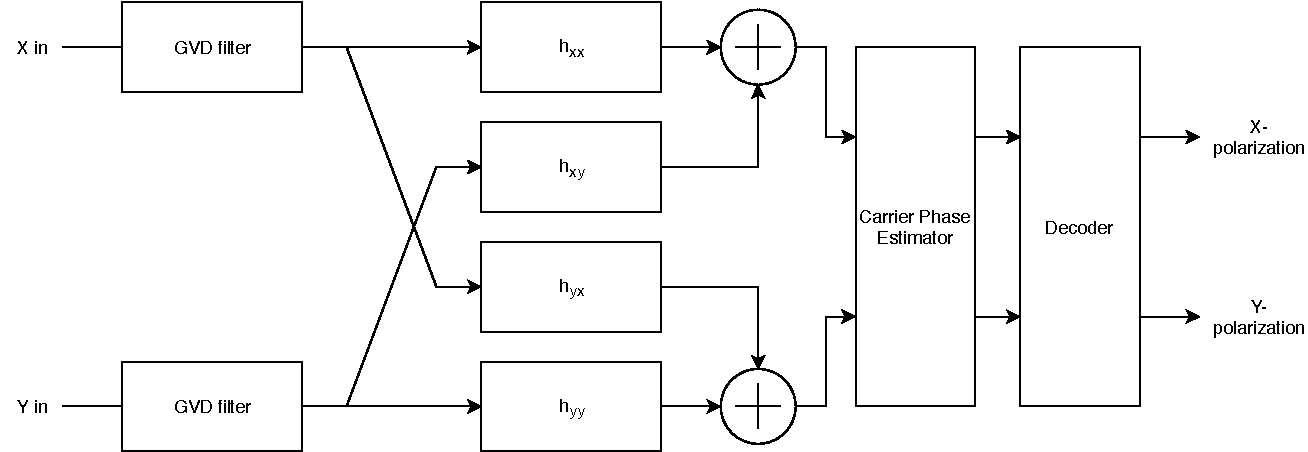
\includegraphics[width=\linewidth]{Thesis/images/dsp.pdf}
    \caption{DSP chain in optical coherent receiver}
    \label{fig:dsp}
\end{figure}

First, GVD is compensated for in a fixed filter. Then, all other linear impairments are compensated in a structure called butterfly structured finite impulse response (FIR) filters. These filters are adaptive since compensated impairments like PMD vary quickly over time and are stochastic. The filter tap algorithm used can exploit the property that incoming signals have a constant energy level. However, this Constant Modulus Algorithm (CMA) is only possible in modulation schemes with constant modulus, like M-ary PSK. The decision-directed least mean squared (DD-LMS) algorithm can be deployed on modulation schemes with varying complex moduli. This algorithm updates the filter taps based on the error difference between the latest estimation and the actual received bit. This algorithm works by a training sequence of symbols and providing the correct symbols to the receiver side such that it can learn how the filter taps should be set. The equations of the algorithm look as follows: %todo reference 57 of Coherent detection
\begin{align}
    h_{xx}(n+1) &= h_{xx}(n) + \mu e_{X}(n)E_x(n), \label{dd-lms}\\
    h_{xy}(n+1) &= h_{xy}(n) + \mu e_{X}(n)E_y(n),\\
    h_{yx}(n+1) &= h_{yx}(n) + \mu e_{Y}(n)E_x(n),\\
    h_{yy}(n+1) &= h_{yy}(n) + \mu e_{Y}(n)E_y(n), \label{dd-lms2}
\end{align}
where n is the symbol iteration number, $\mu$ is the step-size, $e_{X}$ and $e_{Y}$ are the error signals, and $E_x$ and $E_y$ are the energies of all the included past symbols. $e_{X}$ and $e_{Y}$ are defined to be the difference between the energy of respectively the in-phase and quadrature signal components and the expected in-phase and quadrature components, which are provided in training mode.

Afterwards, the carrier phase is recovered. This can be done with the M-th viterbi-viterbi algorithm\cite{coherent_detection,viterbi}, which takes the symbols to the M-th power and divides with M to get rid of the phase modulation and only output the residue unwanted carrier phase offset. Alternatively, a single stage or two-stage blind phase search (BPS) algorithm can be used. After carrier phase compensation, the signal can finally be decoded and all information can be extracted.

\section{Machine learning techniques}
Machine learning is a popular subset of the scientific field of Artificial Intelligence. Machine learning is a relatively new concept and has a variety of practical applications. The concept of machine learning is that an computational algorithm is formed, which is not explicitly programmed, but is rather incrementally formed with the use of data. This data is called the training data and this data adapts the current algorithm into a better performing algorithm in small steps using the principles of statistics. Because machine learning is based on statistics and not on predefined behaviour, machine learning is regarded as a black box solution to algorithmic problems.

Machine learning can be categorized into three different paradigms of learning: supervised learning, unsupervised learning and reinforcement learning. In supervised machine learning, current predictions after data processing are compared to the correct values. Using the difference of the two, the algorithm is adapted. An example of supervised learning is inputting pictures of handwritten numbers, outputting a predicted value and comparing it to the actual value of the written number. Another, more complex field of machine learning is unsupervised learning, which does not use the correct values but rather classifies the data into discrete classes that show similar features. This is useful to distinguish (unlabeled) data into categories. An example is classifying pictures of zoo animals into categories that represent the different animals in the pictures. Lastly, reinforcement learning is a type of learning that tries to learn how to get the best reward out of a situation in an environment. This action does not have to be optimal in the current situation, but has to earn the highest cumulative reward. Therefore, there is a trade-off between using current information and thus getting a quick reward and exploring new information. An example of reinforcement learning is learning to play chess: a certain risk in a chess environment might result in winning the game and thus maximizing cumulative reward.

Machine learning solutions can be useful when there are complex statistical problems with clear  input and output data that involve decision making, categorizing data or giving predictions. After training, the developed algorithm to perform this task is abstract (black box solution).

\subsection{Artificial neural networks}
Within supervised machine learning, artificial neural networks are commonly used to develop solutions. This technique is inspired by how the networks of neurons in animal brains work. An example of an artificial neural network is given in Fig.~\ref{fig:nn}. In the example network, the input values, $x_n$ for $n\in \{1..5\}$ are multiplied with edge weights that are incorporated in a weight matrix $W^{(1)}$. A bias $b^{(1)}$ is added to this resulting vector. To keep the elements in this vector within certain bounds and to add non-linearity to the neural network, the elements of the vector are first sent through an activation function. A commonly used activation function is the Sigmoid function $\sigma(x) = \frac{1}{1+e^{-x}}$. The elements of the resulting vector are the nodes of the first hidden layer in the neural network, $a_n^{(2)}$ for $n\in \{1..3\}$. Mathematically, the next layer $a^{(n+1)}$ is calculated by 
\begin{equation}
    a^{(n+1)} = \sigma\left(a^{(n)}W^{(n)}+b^{(n)}\right),
\end{equation}
where $n$ is a layer number. To account for the first and last layer, $a^{(1)} = x$ is the input layer, and $a^{(m)} = h$ is the output layer, where $m$ is the amount of hidden layers in the network + 2. The output values are compared with the correct labels with a loss-function. Based on the chosen loss-function, the network weights and biases are adapted to more suitable values through a operation called backpropagation\cite{backpropagation}, which closely resembles the DD-LMS algorithm from equations \ref{dd-lms}-\ref{dd-lms2}.

\begin{figure}
    \centering
    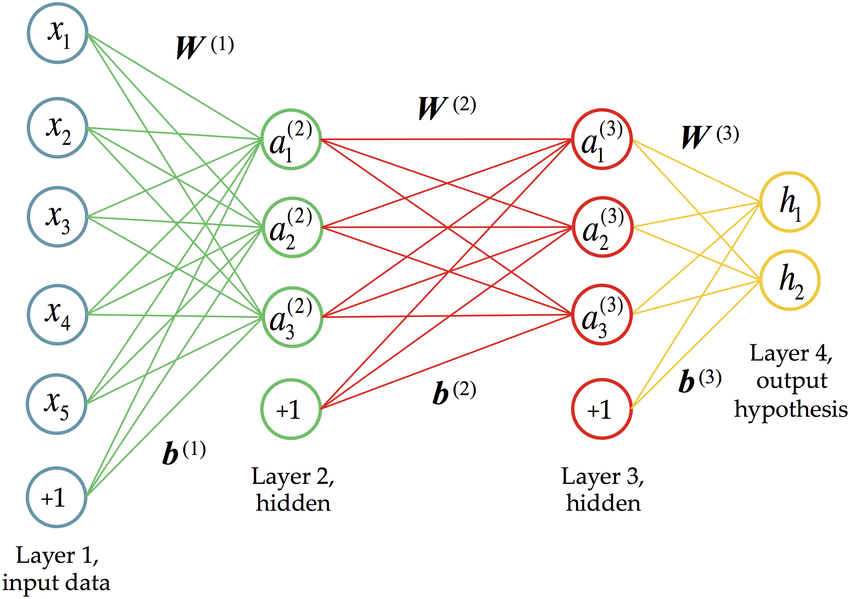
\includegraphics[width=\linewidth]{Thesis/images/nn.png}
    \caption{Example of artificial neural network}
    \label{fig:nn}
\end{figure}

The performance of the neural network is dependent on numerous factors. Some of these factors are:
\begin{itemize}
    \item The amount of hidden layers
    \item The number of nodes within a hidden layer
    \item The activation function
    \item The amount of training steps
    \item How representative the training data is
    \item How balanced the training data is
    \item Learning rate when updating the weights
\end{itemize}

\subsection{Recurrent neural networks}
A special class of neural networks that can deal with data sequences are recurrent neural networks (RNN). These networks differ from normal neural networks in a way that the previous output is included in the new input. The data is therefore continuously looping through the hidden network and old or intermediate predictions are combined in the input layer of the next iteration. RNNs are most suitable when the input data has sequential behaviour.

However, RNNs have learning problems when the network has to remember data from the past that is too far away due to the vanishing/exploding gradient problem. This problem has been solved in 1997 by a network structure called the Long Short Term Memory (LSTM)\cite{lstm} neural network, which is a special version of a RNN. A schematic of this type of network is shown in Fig.~\ref{fig:lstm}.

\begin{figure}
    \centering
    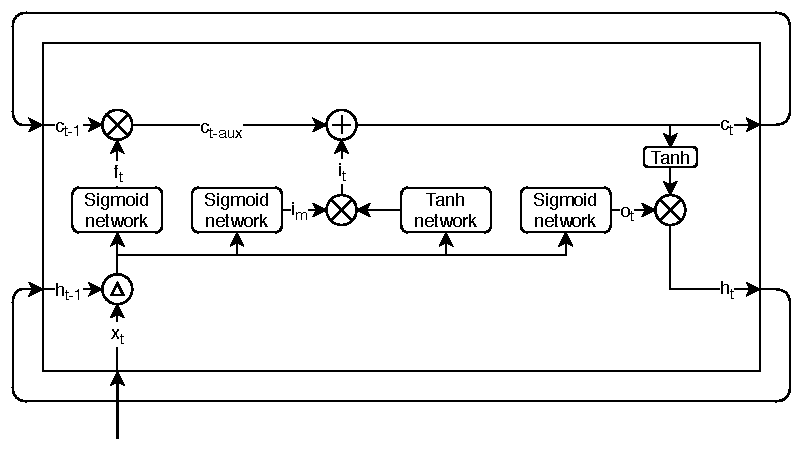
\includegraphics[width=\linewidth]{Thesis/images/lstm.pdf}
    \caption{Schematic depiction of an LSTM. The \textcircled{$\scriptstyle \Delta$} operator is the concatination of the new input with the old output. The \textcircled{$+$} operator is vectorial addition. The \textcircled{$\times$} operator is elementwise multiplication between vectors. Note how the old internal state and output are fed back as new inputs for the next iteration.}
    \label{fig:lstm}
\end{figure}

The network has an internal state $c_t$ which holds remembered information from the past. Every iteration, part of this information is forgotten, added, and outputted, depending on the new input and previous output. First, information is forgotten by element-wise multiplying $c_t$ with a forget vector $f_t$, consisting of values between 0 and 1, a 0 indicating to fully forget information, and a 1 indicating to keep remembering information. This is shown in equation \ref{c_intermediate}. This vector $f_t$ is generated by a network with a Sigmoid activation function. The input of this network is the new input $x_t$ and previous output $h_{t-1}$ of this LSTM iteration. This is shown in equation \ref{forget}. Then, new information is added to $c_t$. To do this, the input (and thus also the previous output) are fed through a network with a $tanh(x) = \frac{e^x - e^{-x}}{e^x + e^{-x}}$ activation function. This information is modulated by a vector $i_{t_{aux}}$ from another Sigmoid driven network as shown in equation \ref{input}. The modulated vector $i_t$ is stated in equation \ref{input_mod}. In equation \ref{new_c} it is shown how the internal state is updated. The output $h_t$ is modulated by the vector $o_t$, which again is the result of a Sigmoid driven network and is shown in equation \ref{output}. The final output $h_t$ is the result of the tanh of the internal state, $tanh(c_t)$, modulated by $o_t$. This is shown in equation \ref{new_h}. 

\begin{align}
    c_{t_{aux}} &= f_t \circ c_{t-1} \label{c_intermediate}\\
    f_t &= \sigma\left(W_fx_t + U_fh_{t-1}+b_f\right) \label{forget}\\
    i_m &= \sigma\left(W_mx_t + U_mh_{t-1}+b_m\right) \label{input}\\
    i_t &= i_m \circ \tanh\left(W_ix_t + U_ih_{t-1}+b_i\right) \label{input_mod}\\
    c_t &= c_{t_{aux}} + i_t \label{new_c}\\
    o_t &= \sigma\left(W_ox_t + U_oh_{t-1}+b_o\right) \label{output}\\
    h_t &= o_t \circ \tanh\left(c_t\right) \label{new_h}
\end{align}

In equations \ref{c_intermediate}-\ref{new_h}, the $t$ subscript denotes the LSTM iteration. $W$ and $U$ respectively denote the weight matrix for the new input $x_t$ and the old input $h_{t-1}$. $b$ is the network bias. Subscripts $f$, $i$, $m$ and $o$ respectively mean "forget", "input", "modulation" and "output". The operator $\circ$ is the elementwise multiplication between vectors.

\section{Machine learning substitution in optical coherent DSP systems}
To incorporate machine learning in the DSP system of the optical coherent receiver, a suitable machine learning structure has to be chosen. To first test if machine learning can be used in the optical receiver, the final part of the receiver, the decoder, has been substituted with a neural network. The rest of the DSP chain remains the same. A schematic depiction of the DSP chain substitution is shown in Fig.~\ref{fig:dsp_linear}. The pseudo-random data has been simulated by the Python framework QAMpy. For this experiment, only Gaussian noise has been added. The parameters of the simulation are shown in Table~\ref{tab:linear}.

\begin{figure}
    \centering
    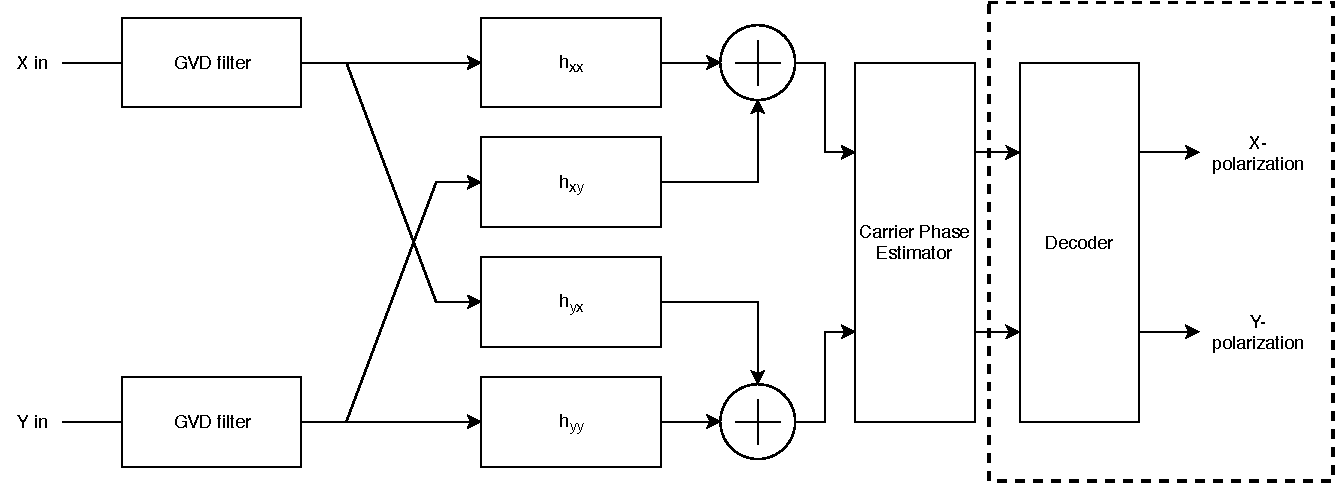
\includegraphics[width=\linewidth]{Thesis/images/DSP_linear.pdf}
    \caption{Machine learning aided DSP chain for QAM decoder experiment. Marked in the dashed rectangle encloses the substituted DSP part}
    \label{fig:dsp_linear}
\end{figure}

\begin{table}
    \centering
    \caption{Used parameters in decoder neural network}
    \label{tab:linear}
    \begin{tabular}{c|c}
        Parameter & Value\\
        \hline
        Modulation scheme & 64-QAM\\
        Generated symbols per polarization & $2^{20}$\\
        SNR & 15\\
        Hidden layers & 1\\
        Hidden nodes & 32\\
        Activation function & ReLU\\
        Sample data per training step & 64\\
        Learning rate & 0.001\\
        Optimizer & Adam optimizer\\
        Loss function & Cross entropy\\
        Amount of training batches & 75\% of $2^{20}/64$ (24576)\\
        Amount of testing batches & 25\% of $2^{20}/64$ (8192)\\
    \end{tabular}
\end{table}

The results are shown in Fig.~\ref{fig:linear}. The different colors show how the decision boundaries of the network look like in the constellation plot. After training, the final achieved accuracy using the test data was 99.9886\%.

\begin{figure}
    \centering
    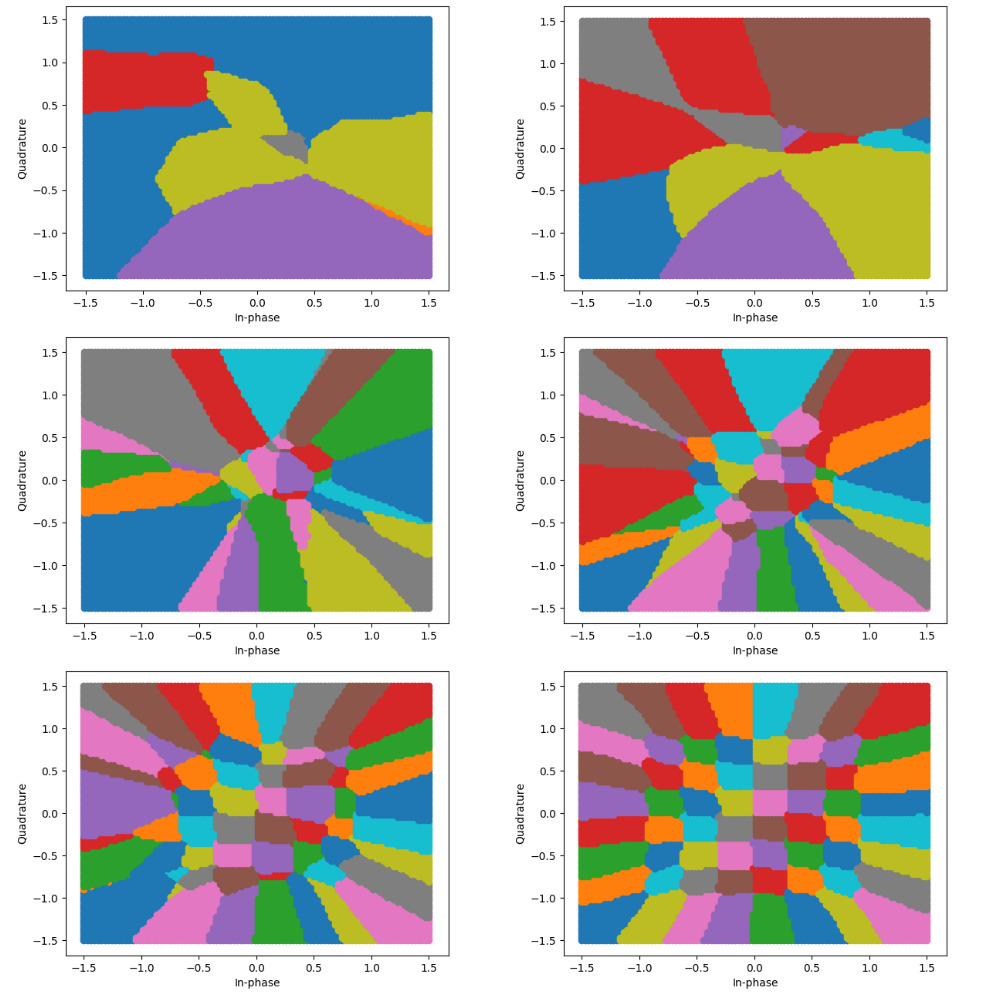
\includegraphics[width=\linewidth]{Thesis/images/linear.jpg}
    \caption{Development of 64-QAM decoder neural network. Upper left after 1 training steps, upper right after 10 training steps, middle left after 300 training steps, middle right after 500 training steps, bottom left after 1000 training steps and bottom right after 24576 training steps}
    \label{fig:linear}
\end{figure}

Decoding the final signals which are only distorted by Gaussian noise is not a practical example of machine learning in an optical receiver. To solve this, more of the receiver DSP has to be included in the machine learning algorithm. Because the conventional way of filtering includes a FIR that uses data from the near past, the machine learning network should also include the past data sequence. Therefore, a suitable machine learning network for replacing the entire DSP chain would be to use an RNN-like structure, such as an LSTM.

To experiment with the unique combination of optical fiber communication and LSTMs, an environment was created as depicted in Fig.~\ref{fig:combi}. The two used frameworks are QAMpy and PyTorch: QAMpy to generate pseudo-random complex symbols and artificial impaired symbols, and PyTorch to implement the recovery network. The output of the first block are the original symbols and the impaired symbols, which are converted in respectively an 3D and 4D tensor. This first tensor contains per batch a 2D tensor consisting of the final correct bit predictions. The second tensor contains per batch a 3D tensor: a sequence of impaired signal energy levels.

\begin{figure}
    \centering
    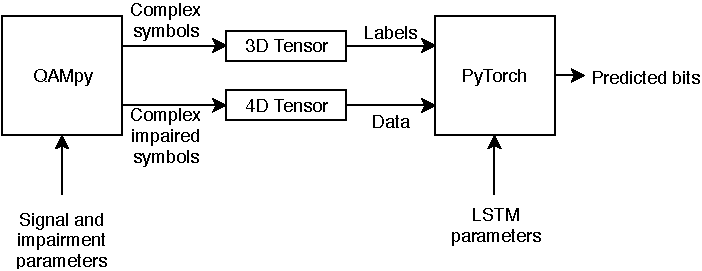
\includegraphics[width=\linewidth]{Thesis/images/framework_combi.pdf}
    \caption{Environment of the conducted experiment}
    \label{fig:combi}
\end{figure}

To compare the structure with the conventional receiver as in Fig.~\ref{fig:coherent_detection}, the virtual environment can be regarded as shown in Fig.~\ref{fig:frameworks}, indicating which parts are implemented by which framework. The medium impairments made in QAMpy are however artificial and no real polarization and phase diversity homodyne receiver is implemented, so the shown components in the right part of Fig.~\ref{fig:frameworks} are modeled artificially and in a digitized way.

\begin{figure}
    \centering
    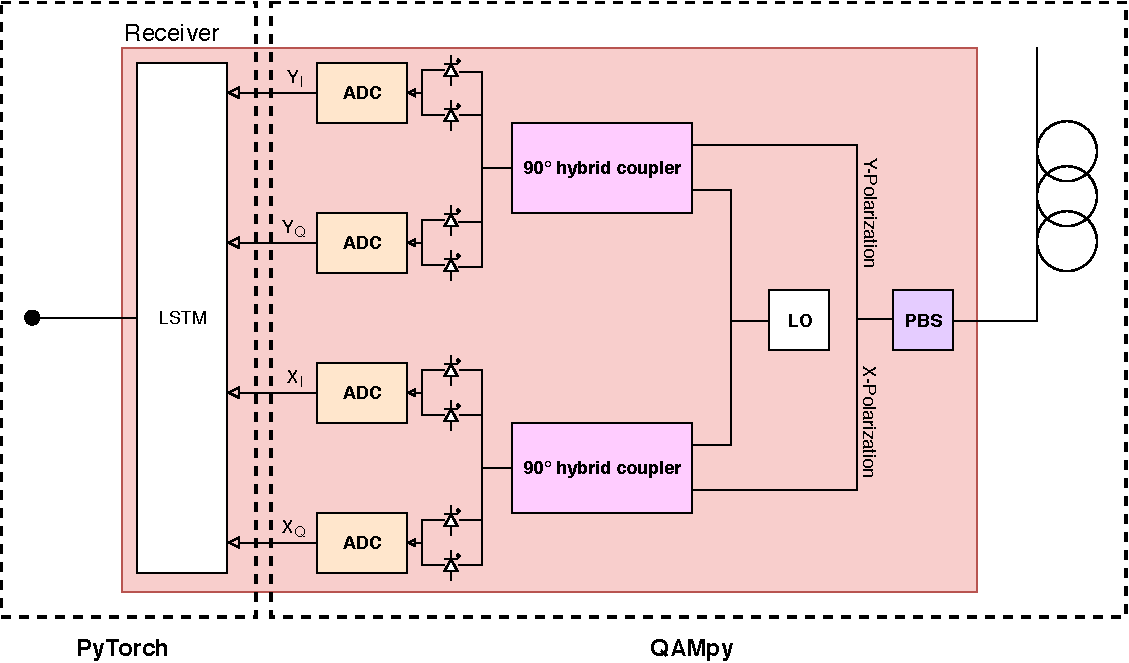
\includegraphics[width=\linewidth]{Thesis/images/PyTorch_QAMpy.pdf}
    \caption{Receiver structure for experiment}
    \label{fig:frameworks}
\end{figure}

The amount of iterations through the LSTM is defined as the length of the training sequence L. The four input nodes of the LSTM are the in-phase and quadrature energy levels of both polarizations. The N output nodes $h_k, k\in\{1..L\}$ are the predicted bit of both polarization, where N is
\begin{align}
    N = 2\log_2(M),
\end{align}
in which M is the alphabet size of the modulation. How the weights of the LSTM are trained is depicted schematically in Fig.~\ref{fig:lstm_training}.

The network trains by receiving a discrete sequence of input data and for every pair of symbols, it outputs a prediction of the N bits. Only at the last prediction, the LSTM gets feedback on what the actual last N bits should have been and updates all its weight matrices and biases based on the loss function. The weight updating algorithm is backpropagation. 

\begin{figure}
    \centering
    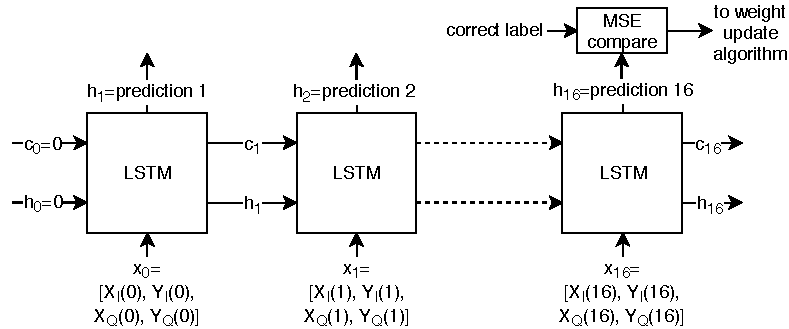
\includegraphics[width=\linewidth]{Thesis/images/lstm_training.pdf}
    \caption{Training of an LSTM, where the sequence length L is 16}
    \label{fig:lstm_training}
\end{figure}

After training, an indefinite discrete sequence of impaired symbol energy levels can be sent through the network. The network gives a prediction for every given input and is no longer dependent on a predefined sequence length.

\section{Experiment}
In this section, the simulated experiment is described. First, the transmitted signal is discussed, whereafter the impairments and the received signal are addressed. Then, the recovery network is explained.

After the simulated experiment, the experiment with real world data from a optical fiber lab is discussed.

\subsection{Transmitted signal}
The parameters of the data and signal impairments are shown in Table~\ref{tab:parameters}. The resulted signal constellation of the original signal is given in Fig.~\ref{fig:sig}. For the X-polarization of this original signal, the first 16 symbols are shown in a 3D time-plot in Fig.~\ref{fig:sig_time}.

\begin{table}
    \centering
    \caption{Used parameters of generated test data}
    \label{tab:parameters}
    \begin{tabular}{c|c}
        Parameter & Value\\
        \hline
        Modulation & QPSK\\
        Amount of symbols per polarization & $2^{20}$\\
        Symbol rate & 25GBd\\
        Pulse shaping & Root raised cosine\\
        $\beta$ of RRcos & 0.1\\
        SNR & 15\\
        $\theta$ of PMD & $\frac{\pi}{5}$\\
        $\tau_{DGD}$ of PMD & 40ps\\
        Linewidth of lasers & 1MHz\\
        Frequency offset between lasers & 1MHz\\
    \end{tabular}
\end{table}

\begin{figure}
    \centering
    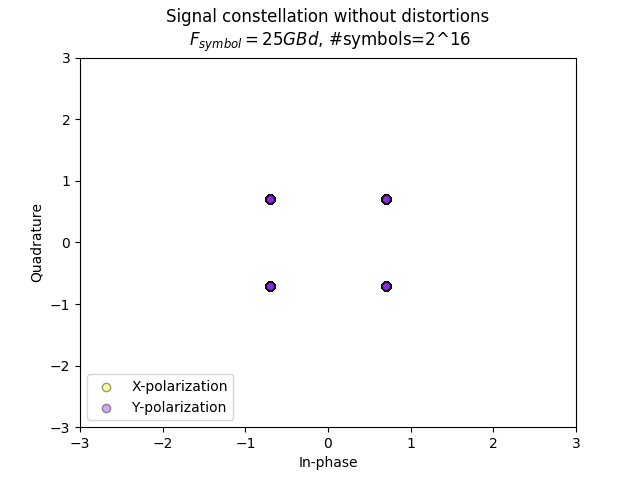
\includegraphics[width=\linewidth]{Thesis/images/sig.png}
    \caption{Signal constellation of original signal}
    \label{fig:sig}
\end{figure}

\begin{figure}
    \centering
    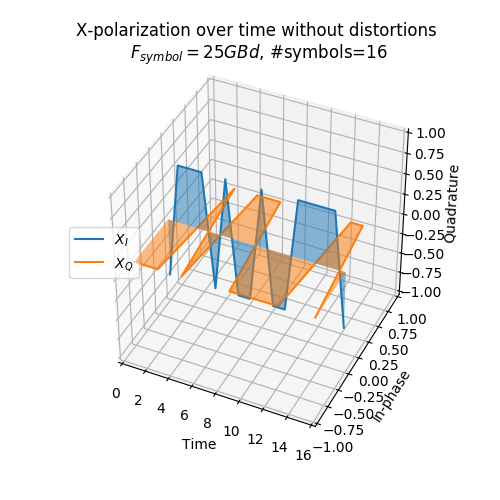
\includegraphics[width=\linewidth]{Thesis/images/sig_time}
    \caption{Time plot for X-polarization of original signal}
    \label{fig:sig_time}
\end{figure}

To limit the required bandwidth of the signal, the signal is pulse-shaped with a root raised cosine filter with a roll-off factor $\beta$ of 0.1. After pulse shaping, the signal constellation and time plot are slightly distorted. The resulting signal constellation and X-polarization time plots are shown in respectively Fig.~\ref{fig:sig_shaped} and Fig.~\ref{fig:sig_shaped_time}. This signal is the signal that is sent by the transmitter.

\begin{figure}
    \centering
    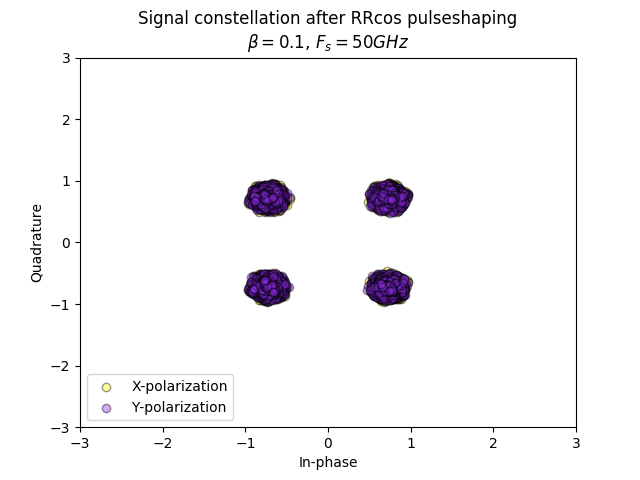
\includegraphics[width=\linewidth]{Thesis/images/sig_shaped}
    \caption{Signal constellation of pulse-shaped original signal}
    \label{fig:sig_shaped}
\end{figure}

\begin{figure}
    \centering
    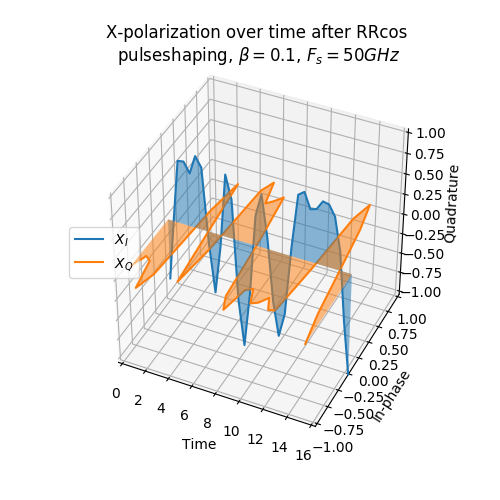
\includegraphics[width=\linewidth]{Thesis/images/sig_shaped_time}
    \caption{Time plot for X-polarization of pulse-shaped original signal}
    \label{fig:sig_shaped_time}
\end{figure}

\subsection{Received signal}
While transmitting the bandlimited signal, the signal is inevitably impaired by the effects as discussed in section \ref{ch:Medium}. These impairments were artificially added to the transmitted signal. The resulting signal constellation plots for the incrementally added impairments can be seen in Fig.~\ref{fig:sig_agwn}-\ref{fig:sig_agwn_pmd_phase_freq}. First, additive Gaussian white noise was added (Fig.~\ref{fig:sig_agwn}). Then, PMD impairments were included (Fig.~\ref{fig:sig_agwn_pmd_phase}). Finally, phase noise (Fig.~\ref{fig:sig_agwn_pmd}) and frequency offset (Fig.~\ref{fig:sig_agwn_pmd_phase_freq}) were added. This final plot is what the receiver picks up after the ADCs and is input for the recovery neural network.

\begin{figure}
    \centering
    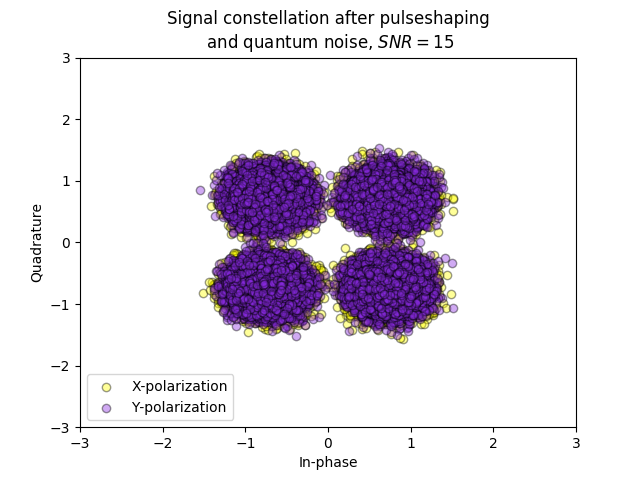
\includegraphics[width=\linewidth]{Thesis/images/sig_agwn}
    \caption{Signal constellation of received signal, impaired by AGWN}
    \label{fig:sig_agwn}
\end{figure}

\begin{figure}
    \centering
    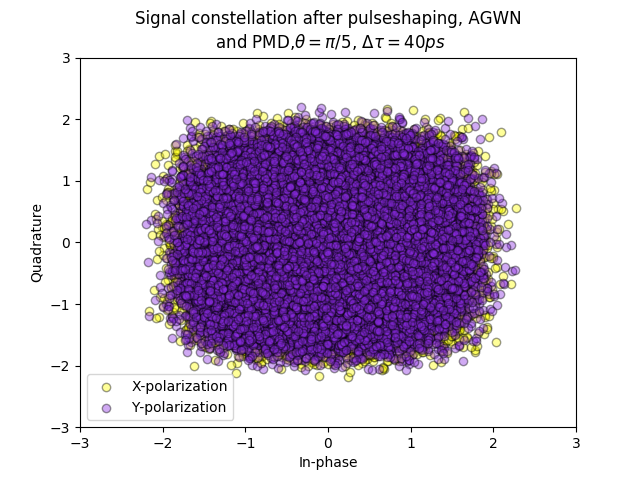
\includegraphics[width=\linewidth]{Thesis/images/sig_agwn_pmd}
    \caption{Signal constellation of received signal, impaired by AGWN and PMD}
    \label{fig:sig_agwn_pmd}
\end{figure}

\begin{figure}
    \centering
    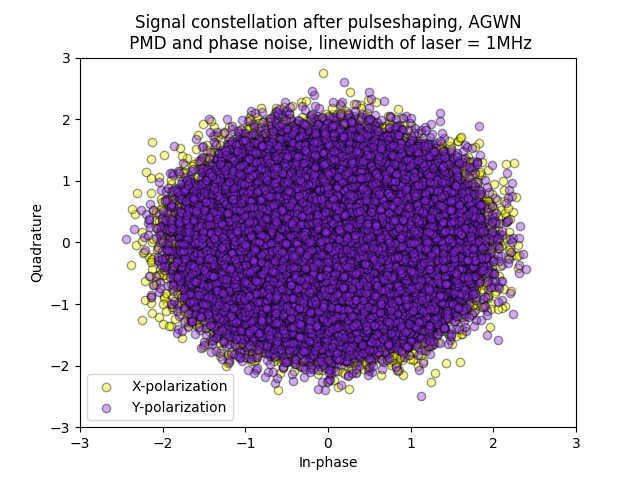
\includegraphics[width=\linewidth]{Thesis/images/sig_agwn_pmd_phase}
    \caption{Signal constellation of received signal, impaired by AGWN, PMD and phase noise}
    \label{fig:sig_agwn_pmd_phase}
\end{figure}

\begin{figure}
    \centering
    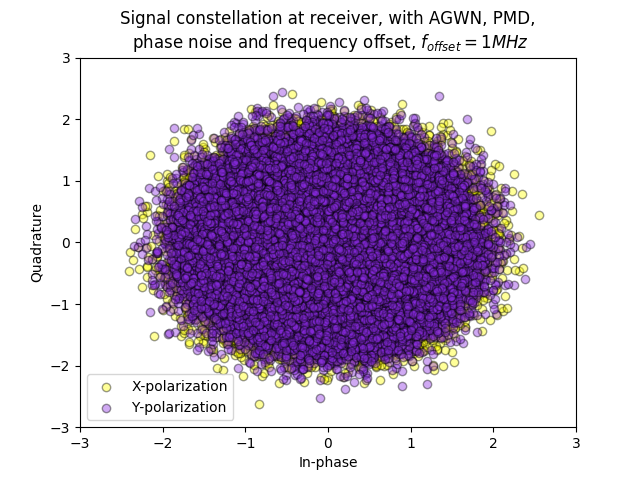
\includegraphics[width=\linewidth]{Thesis/images/sig_agwn_pmd_phase_freq}
    \caption{Signal constellation of received signal, impaired by AGWN, PMD, phase noise and frequency offset}
    \label{fig:sig_agwn_pmd_phase_freq}
\end{figure}

\subsection{Recovery network}
To train the network, the training batches were shuffled to increase the balance of the training data. In this way, the network does not overfit on associated noise of the previous sequence, since this is one of the pitfalls of neural network training.

Unfortunately, the neural network did not show results significantly higher than 50\% (random guessing) after fully training and seemed to have an non-decreasing loss function. The reason why this is the case is because no carrier phase estimator is input in the network, which is included is Fig.~\ref{fig:dsp}. Therefore, the network could not filter out impairments like phase noise and frequency offset.

To see if the network would have a better performance with extra carrier phase estimation information, the M-th power viterbi-viterbi was added in the network, but without success. Also, two-stage blind phase search was added, but no improvement to the 50\% accuracy was shown. Why this is the case is because of the 90 degree symmetric nature of QAM in combination with the shuffling of training data batches. The network can find out what the residue carrier phase offset is (viterbi-viterbi or blind phase search algorithm) within a 90 degree quadrant. However, the network cannot know in which quadrant it is located, because no initial conditions in a randomly selected batch sequence are known. These initial conditions are crucial to predict the integer multiple of 90 degree carrier phase offset of the signal. Thus, prediction acts as a random guess and accuracies cannot by definition have a better performance than 50\%. 

To see if the network would perform without the carrier phase estimator, the phase noise and frequency offset impairments were omitted in the simulation. The substitution of the DSP chain is depicted in Fig.~\ref{fig:dsp_sub}. The parameters of the training data and LSTM are given in Table~\ref{tab:lstm}. 

\begin{figure}
    \centering
    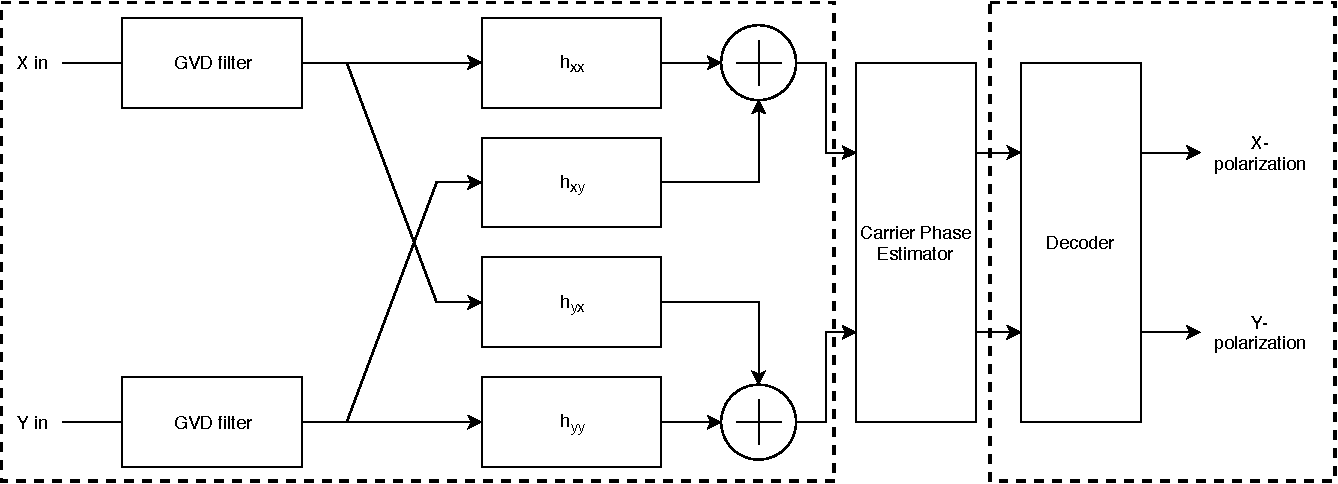
\includegraphics[width=\linewidth]{Thesis/images/DSP_LSTM.pdf}
    \caption{DSP chain substitution by LSTM as marked within dashed boxes}
    \label{fig:dsp_sub}
\end{figure}

\begin{table}
    \centering
    \caption{Parameters of training data and LSTM}
    \label{tab:lstm}
    \begin{tabular}{c|c}
        Parameter & Value\\
        \hline
        Training sequence length & 16\\
        Learning rate & 0.01\\
        Hidden layers & 1\\
        Hidden nodes & 128\\
        Batch size & 128\\
        Training batches/Testing batches ratio & 90\%/10\%\\
        Optimizer & Adam optimizer\\
        Loss function & Mean squared error\\
    \end{tabular}
\end{table}

The graphs of the loss functions for the LSTM for various SNRs is given in Fig.~\ref{fig:loss}. The accuracy graphs of the prediction correctness is given in Fig.~\ref{fig:accuracy}. In all training examples, phase noise and frequency offset were omitted. The final testing data accuracies for the SNR of 30, 15 and 6 were respectively 100\%, 98,5952\% and 83,5871\%.

\begin{figure}
    \centering
    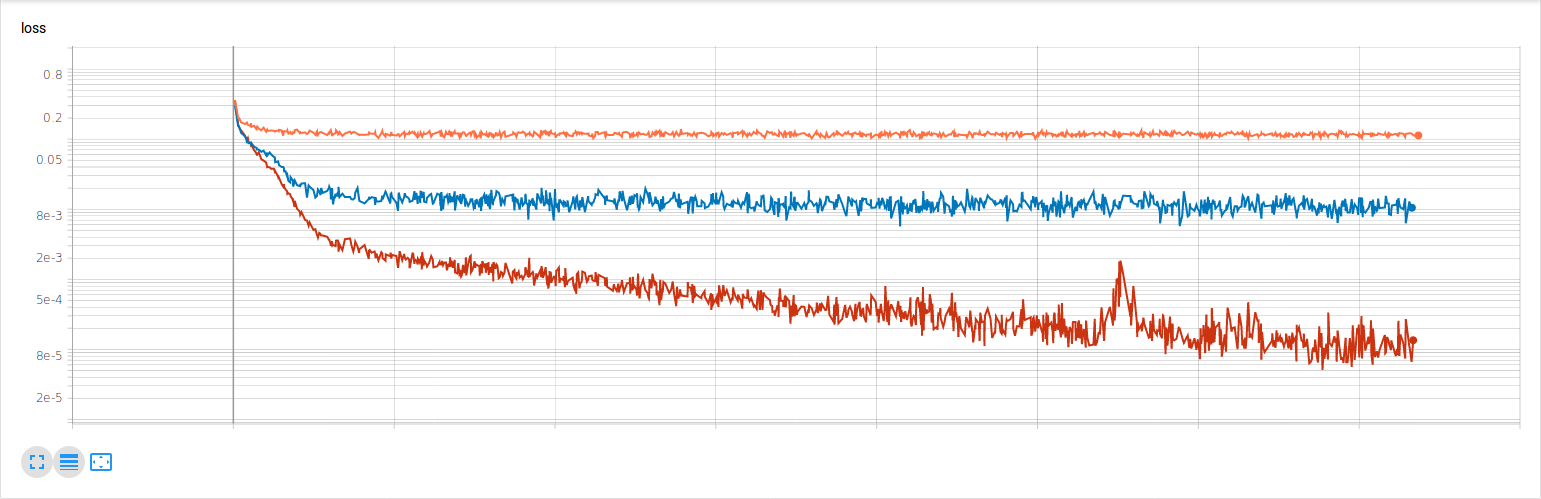
\includegraphics[width=\linewidth]{Thesis/images/loss.png}
    \caption{Loss function of LSTM, red curve: SNR 30, blue curve: SNR 15, orange curve: SNR 6. X-axis depicts the amount of training steps. Logaritmic Y-axis}
    \label{fig:loss}
\end{figure}

\begin{figure}
    \centering
    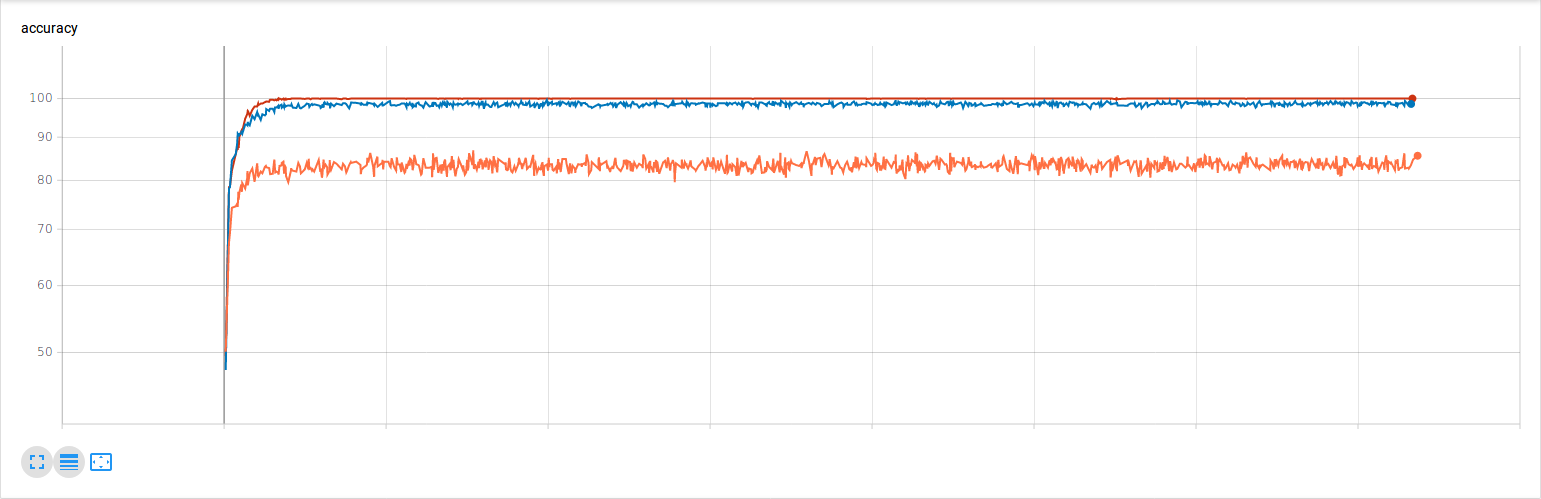
\includegraphics[width=\linewidth]{Thesis/images/accuracy.png}
    \caption{Prediction accuracy of LSTM, red curve: SNR 30, blue curve: SNR 15, orange curve: SNR 6. X-axis depicts the amount of training steps. Logaritmic Y-axis}
    \label{fig:accuracy}
\end{figure}

\subsection{Real data experiment}
To test the LSTM performance with real data, test data from a optical fiber lab was used. The modulation of this data is 8-QAM. 65536 pseudo-random symbols were sent which are pulse-shaped by a root raised cosine filter with roll-off factor $\beta=0.01$. The data was sent once through a standard single mode optical fiber (SSMF) of 75km and was amplified once by an erbium-doped fiber amplifier (EDFA). The frequency offset was separately compensated for, because the network does not have any frequency offset compensating functionality. The input constellation can be seen in Fig.~\ref{fig:input}. The output constellation is shown in Fig.~\ref{fig:output}. The parameters of the training data and the LSTM are given in Table~\ref{tab:real_parameters}. The final obtained accuracy of the prediction network is 83.2145\%.

\begin{figure}
    \centering
    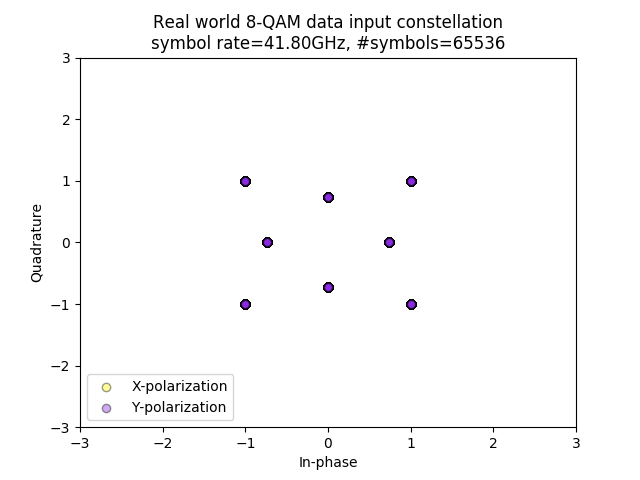
\includegraphics[width=\linewidth]{Thesis/images/real_input.png}
    \caption{Input constellation of real world 8-QAM data}
    \label{fig:input}
\end{figure}

\begin{figure}
    \centering
    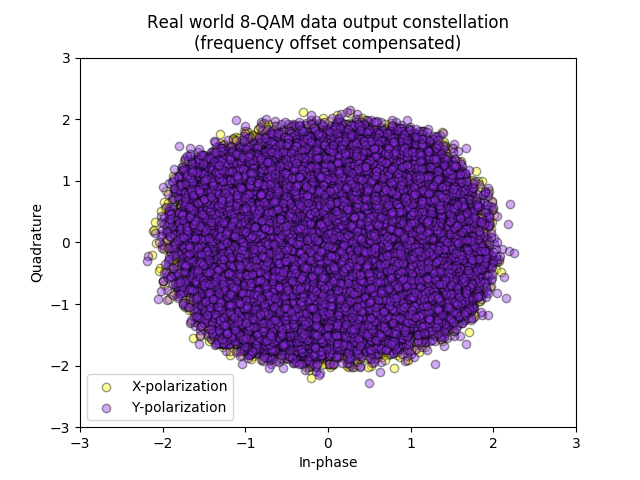
\includegraphics[width=\linewidth]{Thesis/images/real_output.png}
    \caption{Output constellation of 8-QAM signal after 75km of SSMF with one EDFA amplification}
    \label{fig:output}
\end{figure}

\begin{table}
    \centering
    \caption{Parameters of training data and LSTM of real world experiment}
    \label{tab:real_parameters}
    \begin{tabular}{c|c}
        Parameter & Value\\
        \hline
        Training sequence length & 32\\
        Learning rate & 0.02\\
        Hidden layers & 1\\
        Hidden nodes & 128\\
        Batch size & 128\\
        Training batches/Testing batches ratio & 90\%/10\%\\
        Optimizer & Adam optimizer\\
        Loss function & Mean squared error\\
    \end{tabular}
\end{table}

\section{Discussion}
The results of the simulated and real data do not show improvement in comparison with the currently deployed DSP chain hardware. The current DSP chain has a BER of several orders of magnitude lower. However, it is difficult to find out what exactly is the cause of this as neural networks do not show intermediate steps in its predictions. Furthermore, carrier phase estimation is not included in the LSTM and therefore it cannot properly filter out phase noise and frequency offset between the transmitter laser and the local oscillator.

The are some advantages of a machine learning approach to the optical coherent receiver signal recovery problem over the conventional way. One of these advantages is that it is able to filter both linear and non-linear impairments due to the non-linear (Sigmoid) activation function embedded in the network. Furthermore, no knowledge is needed about the transmission line and signal impairments do not have to be modeled correctly, as the network will learn how to deal with any kind of impairment, given a training data sequence of a long enough length. Besides that, all the hardware blocks that are in the conventional receiver DSP can be combined into just a single neural network. Adaptive filters can be replaced by a single fixed and static neural network.

However, there are practical limitations to substituting machine learning techniques in the DSP of an optical coherent receiver. The most important limitation is the enormous increase in computational complexity compared to the low complexity solutions that are currently deployed. Furthermore, improving the BER of the machine learning filter is difficult to do as the model is a black box solution: reverse-engineering a neural network does not give any insight. Also, training sequence has to be performed before real data can be transmitted over the channel. One important limitation is that machine learning techniques are relatively slow and are not yet suitable for high symbol transmission rates unless specifically designed high-speed hardware is made. Lastly, currently, the accuracy is decreased significantly which makes the deployment of machine learning aided DSP unappealing.

\section{Conclusion}
For now, machine learning techniques as a substitute for DSP in optical coherent receivers is not yet feasible. Before this becomes an interesting option, there needs to be more understanding on how to improve the BER of a neural network solution and how the carrier phase estimation can be included in the network. Besides that, the cost of computational complexity in DSP has to decrease before a physical implementation of a neural network is practical.

Besides that, to translate the solution to the optical domain, it first has to be a feasible option to have a phase lock looped system in the optical domain. The received optical signal has to be discretized and is has to be sent through a photonic neural network.

\balance

\bibliographystyle{IEEEtran}
\bibliography{references}

\end{document} 